\documentclass[12pt]{article}
\usepackage{amsmath, amsfonts, amsthm, amssymb, mathtools, cancel}
\usepackage[hidelinks]{hyperref}

\usepackage{times, float}
% \usepackage{fancyhdr}
\usepackage{parskip}
\usepackage{fullpage}
\usepackage{setspace}
\usepackage{bbm}
\usepackage{natbib}
\usepackage{multibib}
\usepackage{booktabs}  % For better table formatting
\usepackage{subfigure}
\bibliographystyle{aea}
\usepackage{subcaption} % Ensure this is in your preamble
\newtheorem{theorem}{Theorem}
\newtheorem{assumption}{Assumption}
\newtheorem{corollary}{Corollary}



%%
%% Stuff above here is packages that will be used to compile your document.

%%%%%%%%%%%%%%%%%%%%%%%%%%%%%%%%%%%%%%%%%%%%%%%%%%%%%%%%%%%


% \setlength{\headheight}{15.2pt}
% \setlength{\headsep}{20pt}
% \pagestyle{fancyplain}
\setlength{\parindent}{20pt}

%%
%% Stuff above here is layout and formatting.
%% Later, you can learn how it all works and adjust it to your liking, or write your own formatting code.
%%%%%%%%%%%%%%%%%%%%%%%%%%%%%%%%%%%%%%%%%%%%%%%%%%%%%%

\singlespacing
%%%%%%%%%%%%%%%%%%%%%%%%%%%%%%%%%%%%%%%%%%%
%% This section contains some useful macros that will save you time typing.
%%

% Using \displaystyle (or \ds) in a block of math has a number of effects, but most notably, it makes your fractions come out bigger.
\newcommand{\ds}{\displaystyle}

% These lines are for displaying integrals; typing \dx will make the dx at the end of the integral look better.
\newcommand{\is}{\hspace{2pt}}
\newcommand{\dx}{\is dx}

% These commands produce the fancy Z (for the integers) and other letters conveniently.
\newcommand{\Z}{\mathbb{Z}}
\newcommand{\Q}{\mathbb{Q}}
\newcommand{\R}{\mathbb{R}}
\newcommand{\C}{\mathbb{C}}
\newcommand{\F}{\mathbb{F}}

%%%%%%%%%%%%%%%%%%%%%%%%%%%%%%%%%%%%%%%%%%%%%%%%%%
\newcommand\independent{\protect\mathpalette{\protect\independenT}{\perp}}
\def\independenT#1#2{\mathrel{\rlap{$#1#2$}\mkern2mu{#1#2}}}

%%%%%%%%%%%%%%%%%%%%%%%%%%%%%%%%%%%%%%%%%%%%%%

% \fancyhead[L]{\textbf{}}
% \fancyhead[C]{\empty}

%%%%%%%%%%%%%%%%%%%%%%%%%%%%%%%%%%%%%%%%%%%%%%%%

\title{The Fixed Allocation Puzzle: Target Date Funds and Active Manager Returns}
\author{Asher Baraban \footnote{I thank Jamie Fogel, Nathan Hendren, and John Nachbar for providing helpful comments. Thanks also to Jonathan Berk for letting me know that using the CRSP mutual funds returns database yields similar results to his more comprehensive database. I thank Shipra Karan and Jack Kelly for their feedback. E-mail: asher.baraban@gmail.com}}


\begin{document}

\maketitle

\begin{abstract}
This paper examines how fixed allocation strategies, where investors maintain a fixed fraction of their portfolio in each asset class, affect asset prices and active manager performance. These strategies, exemplified by popular target date funds and balanced index funds, have grown to trillions of dollars in assets under management, but remain understudied. I develop a theoretical model showing how rebalancing flows due to fixed allocation strategies mechanically create noise trading, potentially benefiting informed investors. Ceteris paribus, the model predicts that as fixed allocation strategies become more common, the rebalance flows should create arbitrage opportunities for active managers. My analysis of 50 years of mutual fund data reveals that active management hasn't successfully capitalized on these opportunities, despite the explosive growth in fixed allocation investing. To understand this pattern, I provide empirical evidence that this result stems from prices increasingly incorporating information over time or a reduction in information frictions. An analysis of insider transactions from SEC Form 4 filings shows low and declining returns to insider trades, evidence in support of market efficiency. While current levels of fixed allocation investing do not significantly impact active investor returns, continued growth may lead to multi-billion dollar transfers from fixed allocation to active investors, with important implications for market efficiency and the design of retirement savings systems.

\textbf{Todos: Does dividend cause exogenous flows?, Redo with rhs as aum*stock - bond returns}


% Contrary to the model's prediction, my analysis of 50 years of mutual fund data reveals that active management has been unable to capitalize on these opportunities despite the explosive growth in fixed allocation investing. To resolve this puzzle, I provide empirical evidence that this unexpected result stems from prices increasingly incorporating information over time. An analysis of insider transactions from SEC Form 4 filings shows declining returns to insider trades. While current levels of fixed allocation investing do not significantly impact active investor returns, continued growth may lead to multi-billion dollar transfers from fixed allocation to active investors, with important implications for market efficiency and the design of retirement savings systems.
\end{abstract}

\doublespacing
\pagebreak

\section{Introduction}
\par Fixed allocation strategies, defined as an investor maintaining a fixed fraction of their portfolio in specific asset classes, are on the rise. Target date funds began to gain significant popularity due to the Pension Protection Act of 2006 \citep{vanguard20years}. By the end of 2022, 68 percent of 401(k) participants hold a target date fund, a popular form of fixed allocation strategy, accounting for 38 percent of all 401(k) assets \citep{ICIFactbook2024}. The growth in fixed allocation strategies is further exemplified by the popularity of Vanguard Target Date Funds, which now manage over \$1 trillion in assets, and the practices of major institutional investors like CalPERS ($>$450B AUM), who adhere to fixed percentage target asset allocations. A key feature of this strategy is the requirement for periodic trading as the relative prices of the asset classes change to maintain the target portfolio weights, a process known as rebalancing. Independent of fundamentals, these mechanical trades could theoretically create arbitrage opportunities for informed investors. This paper uses theory and empirics to study the potential transfers from fixed allocation investors to active managers. 

\par While classical portfolio theory suggests that exposure to the risky asset should be updated frequently to reflect changing market conditions, in practice, many investors adhere to fixed allocations. This behavior may stem from a lack of expertise in continuously reassessing market conditions or from having comparative advantages elsewhere. The model demonstrates how rebalance trades, necessary to maintain fixed allocations, could create exploitable flows in asset markets. These flows may generate profit opportunities for sophisticated market participants with private information. Rebalancing informed by stale beliefs creates a form of noise trading that could be exploited by counterparties with superior knowledge of prices. Essentially, fixed allocation investors act as na\"{\i}ve market makers, increasing liquidity and thus enhancing profitability for those who can identify mispricings. Importantly, sophisticated investors can only profit if mispricings exist.

\par To capture these dynamics, I model a scenario where a mean-variance investor rationally executes a fixed allocation strategy in the presence of another investor with private information. This framework clarifies how private information flows into market prices and creates an equilibrium between active and fixed allocation investing strategies. The model predicts that as the level of wealth managed in fixed allocation strategies grows, so too should the profitability of informed trading. This theoretical approach provides a testable prediction: holding private information quality and market responsiveness fixed, the rise of fixed allocation investing should benefit the performance of active asset managers.

\par To test the prediction of the theoretical model, I first analyze active mutual fund returns over the past 50 years and estimate the performance of each mutual fund over its benchmark portfolio. I use this analysis to gauge if fixed allocation investors are in fact giving up returns to active managers with superior information. If rebalancing creates opportunities for active investors, mutual fund managers should be capitalizing over this time period. I find that mutual funds have not taken advantage of this growth in fixed allocation strategies.

\par Since active managers need private information to produce excess returns, I next analyze private information quality. At its core, a mutual fund return can be decomposed into two components 1) private information quality and 2) market responsiveness, i.e. the change in market price from trading. To measure private information quality, this paper examines returns to insider purchases reported on SEC Form 4 filings. There are two reasons for this approach. First, if prices do not fully incorporate relevant information, company insiders with knowledge of their firm's underlying value should be able to accurately estimate the fair price of the firm, and trade to exploit mispricings. Second, insider transactions possess two key properties that make them a suitable proxy: they are relatively small in size and are executed before public disclosure by the SEC, minimizing their market impact. Consistent with my results on mutual fund performance, I find that the returns of insider transactions have eroded over this period. Moreover, the analysis of insider transactions provides evidence for the theoretical intuition that sophisticated investors can only profit if there are mispricings. 

\par Together, these empirical findings suggest that the rebalance trade has not led to large transfers from fixed allocation investors to active investors due to a fundamental change in the pricing of the market. The core intuition is that fixed allocation investors only create transfers to active managers if prices do not efficiently incorporate information. In essence, the massive rise in fixed allocation investing has not yet created favorable conditions for active managers because prices have become more accurate. However, if the continued rise in fixed allocation investing impedes the efficient incorporation of private information into prices, the rebalance trade could lead to billions of dollars in lost returns in retirement accounts.

\subsection{Related Literature}

\par This paper contributes to several strands of literature in finance and asset pricing. The literature on fixed allocation strategies, particularly target-date funds, has primarily focused on their design and investor outcomes. \citet{MitchellUtkus2020} examine the adoption and impact of target-date funds in 401(k) plans. More recently, \citet{ParkerSchoarSun} investigate the effect of fixed allocation ownership on individual stock returns. However, the effect of fixed allocation strategies on the performance of active managers remains underexplored.

\par My theoretical model builds on the seminal work of \citet{MILGROM198217}. I develop a model with demand for hedging to circumvent the no-trade theorem, allowing it to mirror the reality of massive trading volumes. This approach also relates to the literature on market efficiency, such as \citet{Grossman1980}, by examining how different investor types affect the incorporation of information into prices.

\par The extensive literature on active mutual fund performance, including seminal works by \citet{Jensen1968} and \citet{Carhart}, has generally found little evidence of persistent outperformance. More recently, \citet{BERK2015} argue that the lack of outperformance after fees is consistent with competition. They conclude that mutual fund managers are in fact skilled. \citet{CFM} find that mutual fund managers' investments in firms where they have a social connection outperform. My analysis of mutual fund returns builds on the value-added methodology of \citet{BERK2015} and develops the profitability of insider trades as a proxy for private information, a determinant of mutual fund performance.

\par Finally, my use of insider trading data in this manner builds on a large literature including \citet{Seyhun1998} and \citet{PIOTROSKI}, who demonstrate the profitability and information content of insider trades. I extend this literature by using insider trading returns as a proxy for the changing landscape of private information in markets.

\par By integrating these strands of literature, this paper provides an examination of how the growth of fixed allocation strategies affects market dynamics, information efficiency, and the performance of active managers, contributing to our understanding of the implications of a growing portfolio strategy in the retirement accounts of everyday Americans.


\par The rest of this paper proceeds as follows. Section \ref{sec:theory} presents a setting, where an investor rationally maintains a fixed allocation over time. Section \ref{sec:ramifications} presents the trading implications of maintaining a fixed allocation. It also quantifies the potential transfer from fixed allocation investors' rebalancing to informed investors. Section \ref{sec:empirics} tests the predictions of the model. Section \ref{sec:conclusion} concludes.

\section{Theory} \label{sec:theory}

This section first reviews the classical portfolio choice models, which are the initial motivation for implementing a fixed allocation strategy (portfolio choices independent of wealth). However, carrying out a fixed allocation strategy requires trading in response to market moves. To rationalize this trading with the \citet{MILGROM198217} no trade theorem, I develop a setting with demand for hedging, which motivates trade. The primary result
is that with sufficient uncertainty about the counterparty's motivation to trade (hedging or information asymmetry), it is rational to carry out the fixed allocation strategy.

\subsection{Classical Motivation for a Fixed Percent Allocation}

\par The prevalence of fixed allocation strategies in investment portfolios can be rationalized through classical portfolio theory. This section outlines several classic models of portfolio choice that provide theoretical support for the adoption of such strategies by individual investors and institutions.

\citet{campbell2002strategic} demonstrate that an investor with Constant Relative Risk Aversion (CRRA) utility, faced with allocating between a lognormally distributed risky asset and a risk-free asset, optimally chooses a weight on the risky asset, whose return I denote by R, as:
\begin{equation}
\omega^* = \frac{\log E[R] - \log(R_f)}{\gamma \operatorname{Var}(\log(R))}
\end{equation}
where $R_f$ is the risk-free return and $\gamma$ is the coefficient of relative risk aversion. Similarly, the classic Merton share \citep{Merton} prescribes a portfolio rule of:
\begin{equation}
\omega^* = \frac{E[R] - R_f}{\gamma \operatorname{Var}(\log(R))}
\end{equation}

The same principle emerges in the classical mean-variance framework. Consider an investor with a utility function that trades off linearly between expected return and variance:

\begin{equation}
U(r_p) = E[r_p] - \frac{\gamma}{2}\operatorname{Var}(r_p)
\label{eq:mean_var}
\end{equation}
where $r_p = \omega(r-r_f) + r_f$ is the portfolio return, $r$ is the return on the risky asset, and $r_f$ is the risk-free rate. The investor's optimization problem is:
\begin{align*}
    \arg \max_{\omega \in \R} U(r_p) &= \arg \max_{\omega \in \R} \left\{ E\left[\omega (r - r_f) + r_f\right] - \frac{\gamma}{2}Var\left(\omega (r-r_f) + r_f\right)\right\} \\
    &= \arg \max_{\omega \in \R} \left\{ \omega (E[r] - r_f) + r_f  - \frac{\gamma}{2}\omega^2 Var\left(r)\right)\right\}
\end{align*}
The first-order condition yields:
\begin{equation}
\omega^* = \frac{E[r] - r_f}{\gamma \operatorname{Var}(r)}
\end{equation}

Crucially, in all three related formulations, the optimal fraction invested in the risky asset at a given time is independent of wealth. However, classical theory would expect that the risky share would change dramatically over time using predictors of future returns like the CAPE ratio \citep{campbell1998valuation}. In practice, the fixed allocation strategy is loosely based on, but does not rigorously uphold the prescription of classical portfolio theory. Na\"{\i}vely, fixed allocation investors decide their expected return and variance expectations as long term averages of historical market returns, neglecting to incorporate current market information into their return predictions. Fundamentally, there are large difficulties in accurately identifying future market returns, which suggests a rational inattention model where investors resign themselves to some "reasonable" exposure to the risky asset.
In the next section, I present one mechanism that would explain the behavior of fixed allocation investors. The model is fully rational and is based on an investor's inability to decipher the trading motivations of their counterparty. In the setting of the model, an investor maintains a fixed allocation to the risky asset over time matching the empirical observation that trillions of dollars are invested in fixed allocation portfolios.


% This theoretical result provides a rationale for investors to maintain a fixed allocation over time, only if they estimate expected returns and variances as long-term averages of historical data. While risk aversion might evolve throughout the lifecycle, it is reasonable to assume that these changes occur gradually, allowing for extended periods where the risky weight remains unchanged. This theoretical framework aligns with the empirical observation that substantial assets are invested in fixed allocation portfolios.

\subsection{Justification of a Stationary Fraction and Rebalancing}

\par According to the assumptions of the classical mean-variance optimization theory, the fixed allocation strategy along with its associated rebalancing is optimal if an investor's mean and variance expectations are fixed. However, offers to trade can contain information, which should be incorporated into the investor's expectations, leading to differing fractions of wealth invested in the risky asset over time. Simply, each rebalance trade poses a risk of trading against a counterparty with private information. I present a model where a mean-variance investor rationally maintains a fixed allocation in the presence of a counterparty with private information who profits off of a rebalance trade. To do so, I add a wealth shock to the \citet{MILGROM198217} model, which rationally motivates trade. The fixed allocation investor is willing to trade because they get a sufficiently good deal if their counterparty is hedging (wealth shock), which balances out the losses from trading with a counterparty with private information. 

\subsubsection{Environment}
\par I consider a market with two participants: a na\"{\i}ve investor who does not receive private information and an uncharacterized investor who may receive private information or a wealth shock. Both investors are mean-variance investors, i.e., they trade off linearly between mean and variance with shared risk aversion $\gamma$ for simplicity, as per equation \eqref{eq:mean_var}. I present a two period model. In the first period ($t=0$), there is no trade or competition with other investors, but rather an offering with an infinite supply of the risky asset, i.e. perfectly elastic supply. Investors purchase shares at a fixed price $P_0$. The shares have expected return $\mu_0 > 0$ ($P_T > P_0$) and variance $\sigma^2$ at expiry $T$. As a consequence
of there being an expected return $\mu_0$, the expected price at expiry is $P_T$ s.t. $\frac{P_T - P_0}{P_0} = \mu_0$ where $P_0$ is the issuance price.

Therefore, in the first period $(t=0)$, both investors place $\frac{\mu_0-r_f}{\gamma\sigma^2}$ of their wealth in the risky asset (they are mean-variance investors with shared beliefs). For simplicity, I set $r_f = 0$ so \mbox{$\frac{\mu_0-r_f}{\gamma\sigma^2} = \frac{\mu_0}{\gamma\sigma^2}$}. 

\begin{assumption}
\label{assumption:nonzero-cash}
 \( \frac{\mu_0}{\gamma\sigma^2} < 1 \), which means investors are unlevered in period \(t=0\), and they have a nonzero risk-free asset position in period \(t=0\).
\end{assumption}
In the next period $(t=1)$, the uncharacterized investor either receives a private signal about the expiry price or receives an unpredictable wealth shock $L$ (positive or negative). Then, the two investors have the opportunity to execute a trade with one another. I aggregate these two possibilities, a private signal or a wealth shock, to motivate a realistic model of trade.

Section \ref{subsec:wealth_shock} analyzes the case of the wealth shock. Since the case of only a private signal reduces to \citet{MILGROM198217}, section \ref{subsec:combine} analyzes the situation when the uncharacterized investor can receive either a private signal or a wealth shock.

\subsubsection{Wealth Shock (\textit{L})} \label{subsec:wealth_shock}

In the second period ($t=1$), after both investors purchase their desired number of shares and the issuance is over, the uncharacterized investor receives a wealth shock $L$. For notation purposes, $I_N$ will refer to the "na\"{\i}ve" investor who has wealth $W_{N,1}$ and $I_U$ for the "uncharacterized" investor who has wealth $W_{U,1}$ ($W_{i,j}$ refers to the wealth of investor $i$ in period $j$). Before any trading, the wealth of uncharacterized investor is increased by $L$ as shown in equation \eqref{eq:lottery_win}.

\begin{equation}
    W_{U, 1} = W_{U, 0} + L \quad \text{s.t.} \quad L \in \left(-W_{U,0}\left(1-\frac{\mu_0}{\gamma\sigma^2}\right), \infty\right)
    \label{eq:lottery_win}
\end{equation}
$L$ is constrained to be less than the size of the risk-free position of the uncharacterized investor to avoid the issue of bankruptcy.

I assume the wealth shock does not affect $P_T$, the expected price at expiry, or $\sigma^2$, i.e., $L \independent P_T$ and $L \independent \sigma^2$. Let $\mu_t = \frac{P_T - P_t}{P_t}$ denote the expected return on the risky asset at a given price $P_t$. I assume that $\sigma^2$ stays constant throughout all periods. I now derive the amount each investor wants to trade to compute the new equilibrium price for the market to clear, which informs the $\mu$ going forward (must stay constant for the fixed allocation investor). I assume that there is one opportunity to trade one bulk amount of shares. Intuitively, because of the wealth shock, the sophisticated investor wants to own more of the risky asset if $L>0$ and less if $L<0$.

I first write down the wealth of each investor conditional on the price in the second period $P_1$ before any trades occur.

\begin{equation}
    W_{U, P_1} = \underbrace{W_{U,0}\frac{\mu_0}{\gamma\sigma^2} \left(\frac{P_1}{P_0}\right)}_\text{Risky Position} + \underbrace{W_{U,0}\left(1-\frac{\mu_0}{\gamma\sigma^2} \right)}_\text{Cash Position} + L
    \label{eq:unchar_wealth}
\end{equation}

\begin{equation}
    W_{N, P_1} = \underbrace{W_{N,0}\frac{\mu_0}{\gamma\sigma^2} \left(\frac{P_1}{P_0}\right)}_\text{Risky Position} + \underbrace{W_{N,0}\left(1-\frac{\mu_0}{\gamma\sigma^2} \right)}_\text{Cash Position}
    \label{eq:naive_wealth}
\end{equation}
Equations \eqref{eq:unchar_wealth} and \eqref{eq:naive_wealth} show the wealth of the uncharacterized and na\"{\i}ve investor respectively after the wealth shock. Risky position refers to the portion of the investor's portfolio held in the risky asset, and cash position refers to the portion of the investor's portfolio held in the risk-free asset.

After the wealth shock, the uncharacterized investor no longer holds her ideal fraction of her wealth in the risky position. This creates an incentive to trade, as both investors seek to hold a risky position of $\frac{\mu}{\gamma\sigma^2}$. Thus, I can write down each investor's demand function, which is the difference between the investor's desired risky position and their current risky position. Recall, $\mu_i = \frac{P_T-P_i}{P_i}$, the expected rate of return when purchasing at a price $P_i$. Let $P_1$ be the price that the investors agree upon after the wealth shock. 
\begin{equation}
    D_U(P_1) = \underbrace{\frac{\mu_1}{\gamma \sigma^2}W_{U,P_1}}_\text{Desired Risky Position} - \underbrace{\frac{\mu_0}{\gamma \sigma^2}W_{U,0}\left(\frac{P_1}{P_0}\right)}_\text{Current Risky Position}
\end{equation}
$\frac{P_1}{P_0}$ is the adjustment to the investor's current risky position as the price of the asset moves. Next, I substitute in for $W_{U,P_1}$ using equation \eqref{eq:unchar_wealth}.
\begin{equation}
    D_U(P_1) = \frac{\mu_1}{\gamma \sigma^2}\left(W_{U,0}\frac{\mu_0}{\gamma\sigma^2} \left(\frac{P_1}{P_0}\right) + W_{U,0}\left(1-\frac{\mu_0}{\gamma\sigma^2} \right) + L\right) -\frac{\mu_0}{\gamma \sigma^2}W_{U,0}\left(\frac{P_1}{P_0}\right)
\end{equation}
I next substitute in for $\mu_1 = \frac{P_T - P_1}{P_1}$ to reveal all of the $P_1$ terms, so that I can eventually solve for the equilibrium price.
\begin{equation}
    D_U(P_1) = \frac{P_T - P_1}{P_1\gamma \sigma^2}\left(W_{U,0}\frac{\mu_0}{\gamma\sigma^2} \left(\frac{P_1}{P_0}\right) + W_{U,0}\left(1-\frac{\mu_0}{\gamma\sigma^2} \right) + L\right) -\frac{\mu_0}{\gamma \sigma^2}W_{U,0}\left(\frac{P_1}{P_0}\right)
\end{equation}
Distributing through, we can simplify further.
\begin{equation}
    D_U(P_1) = \frac{P_T - P_1}{(\gamma \sigma^2)^2}W_{U,0}\left(\frac{\mu_0}{P_0} + \frac{1- \mu_0}{P_1}\right) + \underbrace{\frac{P_T - P_1}{P_1\gamma\sigma^2}L}_{\text{Shock Demand}} - \frac{\mu_0}{\gamma \sigma^2}W_{U,0}\frac{P_1}{P_0}
    \label{eq:simple_unchar_demand}
\end{equation}
When $P_1 = P_0$, the demand of the uncharacterized investor is just the shock demand term. Note, that this demand function can be negative, which signifies the desire to sell the risky asset. 


% \begin{align}
% D_U(P_1) &= \underbrace{\frac{\frac{P_T-P_1}{P_1}}{\gamma\sigma^2} \left( W_{U,0}\frac{\frac{P_T - P_0}{P_0}}{\gamma\sigma^2} \left(\frac{P_1}{P_0}\right) + W_{U,0}\left(1-\frac{\frac{P_T - P_0}{P_0}}{\gamma\sigma^2} \right) + L \right)}_\text{Desired Risky Position} - \underbrace{W_{U,0}\frac{\frac{P_T - P_0}{P_0}}{\gamma\sigma^2} \left(\frac{P_1}{P_0}\right)}_\text{Current Risky Position} \nonumber \\
% &= \frac{P_T - P_1}{P_1\gamma\sigma^2}W_{U,0}\left(\frac{P_T - P_0}{P_0\gamma\sigma^2}\frac{P_1}{P_0} + 1 - \frac{P_T - P_0}{P_0\gamma\sigma^2}\right) + \frac{P_T - P_1}{P_1 \gamma\sigma^2}L - W_{U,0}\frac{P_T - P_0}{P_0\gamma\sigma^2}\frac{P_1}{P_0} \nonumber \\ \nonumber \\
% &= \frac{\mu_1}{\gamma\sigma^2}W_{U,0}\left(\frac{\mu_0}{\gamma\sigma^2}\frac{P_1}{P_0} + 1 - \frac{\mu_0}{\gamma\sigma^2}\right) + \frac{\mu_1}{ \gamma\sigma^2}L - W_{U,0}\frac{\mu_0}{\gamma\sigma^2}\frac{P_1}{P_0} \nonumber \\ \nonumber \\
% &= \frac{(P_T-P_1)W_{U,0}}{\gamma \sigma^2 P_0} + \frac{(P_T - P_1)(W_{U,0} - W_{U,0}\mu_0 + L)}{\gamma \sigma^2 P_1} - W_{U,0}\mu_0\frac{P_1}{P_0}
% \end{align}
% Note, this demand function can be negative, which denotes supply or the desire to sell the risky asset.

The na\"{\i}ve trader's demand function is identical to equation \eqref{eq:simple_unchar_demand}, but without the lottery term (substituting in the wealth of na\"{\i}ve investor from \eqref{eq:naive_wealth} for the wealth of uncharacterized investor from \eqref{eq:unchar_wealth}).
\begin{equation}
    D_N(P_1) = \frac{P_T - P_1}{(\gamma \sigma^2)^2}W_{N,0}\left(\frac{\mu_0}{P_0} + \frac{1- \mu_0}{P_1}\right) - \frac{\mu_0}{\gamma \sigma^2}W_{N,0}\frac{P_1}{P_0}
    \label{eq:simple_naive_demand}
\end{equation}
The market-clearing price, denoted as $P_1^*$ is the price at which the quantity supplied equals the quantity demanded, represented by the equation below.
\begin{equation}
    D_N(P_{1}^*) = -D_U(P_{1}^*) 
    \label{eq:supply_demand}
\end{equation}
For completeness, in the theoretical appendix (Appendix \ref{sec:theory_appendix}), I derive the market-clearing price $P_1^*$, but I do not need to solve explicitly for $P_1^*$ to place bounds on the relevant solution of $P_1^*$, thereby also bounding $\mu_1^*$.

\begin{theorem}
If $L>0$, $\exists P_1^* \in (P_0, P_T)$.
\label{thm:pos_wealth_shock}
\end{theorem}
\noindent Theorem \ref{thm:pos_wealth_shock} tells us that when there is a positive wealth shock, the next period ($t=1$) price, $P_1$, lies between issuance price, $P_0$, and the expected expiry price, $P_T$
\begin{proof}
    When $L>0$ the following statements hold.
    \begin{itemize}
        \item $D_U(P_0) > - D_N(P_0)$ as $D_U(P_0) = \frac{\mu_0}{\gamma\sigma^2}L$ and $D_N(P_0) = 0$
        \item $D_U(P_T) < -D_N(P_T)$ as $D_U(P_T) = -\frac{\mu_0}{\gamma\sigma^2}W_{U,0}\frac{P_T}{P_0}$ and $D_N(P_T) = -\frac{\mu_0}{\gamma\sigma^2}W_{N,0}\frac{P_T}{P_0}$
    \end{itemize}
    Therefore, by the intermediate value theorem $\exists P_1^* \in (P_0, P_T)$. 
\end{proof}
\begin{theorem}
If $L<0$, $\exists P_1^* \in (0, P_0)$.
\label{thm:neg_wealth_shock}
\end{theorem}
\noindent Theorem \ref{thm:neg_wealth_shock} tells us that when there is a negative wealth shock, the next period ($t=1$) price, $P_1$, lies between 0 and the issuance price, $P_0$.
\begin{proof}
    When $L<0$ the following statements hold.
    \begin{itemize}
        \item $D_U(P_0) < - D_N(P_0)$ as $D_U(P_0) = \frac{\mu_0}{\gamma\sigma^2}L$ and $D_N(P_0) = 0$
        \item $\lim_{P_1 \to 0^+} D_U(P_1) = \lim_{P_1 \to 0^+} \frac{P_T-P_1}{P_1\gamma\sigma^2}W_{U,P_1} - \frac{\mu_0}{\gamma\sigma^2}W_{U,0}\frac{P_1}{P_0} = \infty$
        \begin{itemize}
            \item $W_{U,P_1} > 0$ if $P_1 >0$ as $L \in \left(-W_{U,0}\left(1-\frac{\mu_0}{\gamma\sigma^2}\right), \infty\right)$ and $W_{U,0} > 0$
        \end{itemize}
        \item $\lim_{P_1 \to 0^+} D_N(P_1) = \lim_{P_1 \to 0^+} \frac{P_T-P_1}{P_1\gamma\sigma^2}W_{N,P_1} - \frac{\mu_0}{\gamma\sigma^2}W_{N,0}\frac{P_1}{P_0} = \infty$ as $(1-\frac{\mu_0}{\gamma\sigma^2}) > 0$ by assumption \ref{assumption:nonzero-cash}.
    \end{itemize}
    Therefore, by the intermediate value theorem $\exists P_1^* \in (0, P_0)$. 
\end{proof}

Theorem \ref{thm:pos_wealth_shock} implies that if $L>0$, $\mu_1^* < \mu_0$. Theorem \ref{thm:neg_wealth_shock} implies that if $L<0$, $\mu_1^* > \mu_0$. The essential insight is that a positive wealth shock increases the equilibrium price, which decreases the return going forward. When the investor receives a negative wealth shock the equilibrium price falls, which increases the return going forward. Therefore, in this scenario, the expected return is not constant. In the following section, I demonstrate that incorporating a private signal can stabilize the expected return after trading has occured.
% \begin{align}
% D_N(P_1)&= \frac{P_T - P_1}{P_1\gamma\sigma^2}W_{N,0}\left(\frac{P_T - P_0}{P_0\gamma\sigma^2}\frac{P_1}{P_0} + 1 - \frac{P_T - P_0}{P_0\gamma\sigma^2}\right) - W_{N,0}\frac{P_T - P_0}{P_0\gamma\sigma^2}\frac{P_1}{P_0} \nonumber \\ \nonumber \\
% &= \frac{\mu_1}{\gamma\sigma^2}W_{N,0}\left(\frac{\mu_0}{\gamma\sigma^2}\frac{P_1}{P_0} + 1 - \frac{\mu_0}{\gamma\sigma^2}\right) - W_{N,0}\frac{\mu_0}{\gamma\sigma^2}\frac{P_1}{P_0} \nonumber \\ \nonumber \\
% &= \frac{(P_T-P_1)W_{N,0}}{\gamma \sigma^2 P_0} + \frac{(P_T - P_1)(W_{N,0} - W_{N,0}\mu_0)}{\gamma \sigma^2 P_1} - W_{N,0}\mu_0\frac{P_1}{P_0} \label{eq:naive_demand}
% \end{align}
% If you multiply both sides by $P_1P_0\gamma\sigma^2$ and collect terms, you end up with the quadratic below. Let $W=W_{U,0}+W_{N,0}$.
% \begin{equation}
%     P_1^{*2}\left(-(1+\mu_0\gamma\sigma^2)W\right) + P_1^{*}\left((P_T-P_0+P_0\mu_0)W - LP_0\right) + P_TP_0(W-\mu_0W+L)=0
% \end{equation}
% I simplify further by rewriting $P_T-P_0$ as $P_0\mu_0$. Therefore, $P_T-P_0 + P_0\mu_0 = 2P_0\mu_0$.
% \begin{equation}
%       P_1^{*2}\left(-(1+\mu_0\gamma\sigma^2)W\right) + P_1^{*}\left((2P_0\mu_0)W - LP_0\right) + P_TP_0(W-\mu_0W+L)=0
% \end{equation}
% Substiuting into the quadratic formula.
% \begin{align}
%     P_{1}^* &= \frac{-\left((2P_0\mu_0)W - LP_0\right) \pm \sqrt{\left((2P_0\mu_0)W - LP_0\right)^2 + 4\left((1+\mu_0\gamma\sigma^2)W\right)P_TP_0(W-\mu_0W+L)}}{-2\left((1+\mu_0\gamma\sigma^2)W\right)} \nonumber  \\ \nonumber \\ 
%     &= \frac{-P_0\left(2\mu_0W - L\right) \pm \sqrt{\left(P_0(2\mu_0W - L)\right)^2 + 4\left((1+\mu_0\gamma\sigma^2)W\right)P_TP_0(W-\mu_0W+L)}}{-2\left((1+\mu_0\gamma\sigma^2)W\right)} \label{eq:eq_price}
% \end{align}



% \subsubsection{Private Signal} \label{subsec:private_info}
% Here, I consider the classic \citet{MILGROM198217} setup where there is no hedging demand just asymmetric information. Consider a market with two investors one who receives a private signal and one naive. They both start with the same expectations and have allocations of $\frac{\mu}{\gamma \sigma^2}$ to the risky asset \footnote{Think of $\mu$ as the excess return so we don't have to worry about the risk-free rate.}. In the next period ($t=1$), one investor receives a signal that changes her $\mu$ to $\mu'$. The active investor learns that the expected value of the risky asset at time $T$ is $P'_T \neq P_T$. Explicitly, $\mu' = \frac{P'_T-P_1}{P_1}$ Thus, the active investor goes to trade, but the naive investor is aware that the active investor can receive private information. This leads to the inability to trade following the logic of \citet{MILGROM198217}. Thus, in reality, the naive investor learns the active investor's private signal $P'$. In this case, the expected return $\mu'$ on the risky asset increases or decreases depending on whether $P'_T$ is larger or smaller than $P_T$.

% XX Potentially add this - Still working out how to do this cleanly XX

% In my setting, I verify that there is in fact no trade between these two parties. They both in period ($t=1$) seek to hold $\frac{\mu'}{\gamma \sigma^2}$ of their wealth in the risky asset. With this information, I can write down the demand functions for the unsophisticated investor. Recall that $W_{U,0}$ is the initial wealth of the uncharacterized investor and $W_{U,P_1}$ is the wealth of the uncharacterized investor conditional on the price of the risky asset as defined in equation \eqref{eq:unchar_wealth}, but with $L=0$. 

% \begin{equation}
%     D_U(P_1) = \frac{\mu'}{\gamma \sigma^2} W_{U,P_1} - \frac{\mu}{\gamma \sigma^2} W_{U,0} \left(\frac{P_1}{P_0}\right)
% \end{equation}
% Equivalently, for the naive investor as per equation \eqref{eq:naive_demand}.
% As before we can set supply equal to demand. I next show that at the equilibrium price there will be no trade.  
% \[ D_N(P_{1}^*) = -D_U(P_{1}^*) \]
% What is about to happen is that $P_1^*$ will move so that both parties hold their desired allocation without trade. I set $L=0$ and $\gamma\sigma^2 = 1$ in equation \eqref{eq:eq_price}.

% \begin{align}
%     P_{1}^* &= \frac{-P_0\left(2\mu_0W\right) \pm \sqrt{\left(P_0(2\mu_0W)\right)^2 + 4\left((1+\mu_0)W\right)P_TP_0(W-\mu_0W)}}{-2\left((1+\mu_0)W\right)}
% \end{align}

% XX

\subsubsection{Combining The Wealth Shock and The Private Signal} \label{subsec:combine}
Now, I add in the private signal. In the second period $(t=1)$, the uncharacterized investor either receives a wealth shock or she receives a private signal that the expected price at expiry is $P_S$. Note, if there was no wealth shock, then this situation would reduce to a case of \citet{MILGROM198217}. The na\"{\i}ve investor is unable to discern the trading motivation of the counterparty: a wealth shock or a private signal. When the uncharacterized investor looks to buy shares, $P_S > P_T$ or $L > 0$. When the uncharacterized investor looks to sell shares, $P_S < P_T$ or $L < 0$. Thus, the na\"{\i}ve investor cannot decipher the motivation of the counterparty. The na\"{\i}ve investor is forced to make assumptions about the probability that the counterparty is trading due to a wealth shock or a private signal. If the beliefs satisfy equation \eqref{eq:combine}, the na\"{\i}ve investor is a fixed allocation investor. If the beliefs about the probabilities and corresponding returns stay stable, this justifies the fixed allocation strategy. 

\begin{equation}
\mu_1 = P(\text{Private Signal})\mu_A + P(\text{Wealth shock})\mu_{1}^* = \mu_0
\label{eq:combine}
\end{equation}
In this scenario, the na\"{\i}ve investor will trade as she is unsure of the counterparty's motivation. This uncertainty violates the assumptions of the \citet{MILGROM198217} no trade theorem to rationally motivate trade, in particular, fixed allocation rebalance trades. The takeaway is that rationally, the na\"{\i}ve fixed allocation investor will trade with sophisticated counterparties if there is sufficient hedging demand. Now that we have established the rationality of the fixed allocation strategy, we can focus exclusively on the trades with sophisticated investors. In the following section, I analyze the potential for transfers from fixed allocation investors to informed investors.


\section{Analyzing the Ramifications of the Fixed Allocation Strategy} \label{sec:ramifications}
In section \ref{subsec:execution}, I analyze the implementation of the fixed allocation strategy, detailing the trades a fixed allocation investor must make to maintain their desired allocation. Section \ref{subsec:profit_opportunities} derives the balance sheet process of the fixed allocation investors and quantifies the potential transfers from fixed allocation investors to informed active managers. Together, these sections analyze how theoretically, informed investors could profit off of the rebalance trade.


\subsection{Executing the Fixed Allocation Strategy} \label{subsec:execution}
A fixed allocation investor seeks to maintain a fixed percentage $\omega$ of her wealth $W_{t}$ in the risky asset. When the risky asset moves (changes price) the fixed allocation investor is forced to buy or sell to maintain their desired exposure to the risky asset $\omega$. The demand function for the risky asset is a function of a fixed allocation investor's risky asset position $S_t$ (stock), cash position $C_t$, and their desired risky weight $\omega$. By definition, $W_t = C_t+S_t$. In general, if an investor seeks to have a fixed percentage of their portfolio $\omega$ in the risky asset, their demand function is given below. 
\begin{align}
D(\omega, C_1,S_1) &= \underbrace{\omega(C_1+S_1)}_{\text{Desired Risky Position}} \ \ - \underbrace{S_1}_{\text{Current Risky Position}} \nonumber  \\
&= \underbrace{\left(\omega-\frac{S_1}{S_1 + C_1}\right)}_{\text{Deviation From Desired Fraction}}W_1
\end{align}
\par I now consider the case of a fixed allocation investor who has already achieved their desired asset allocation at time $t=0$, i.e. $S_0 = \omega(W_0) = \omega(S_0 + C_0)$. At time $t=1$, the risky position has a new price such that $S_1 = (1+K)S_0$ where $K$ is the percent change in the stock price. I assume that the risk-free rate is $0$ which implies that $C_1=C_0$. I show the demand function below for this special case. I use the fact that $W_1 = S_1 + C_1 = S_0(1+K) + C_0 = W_0(1+\omega K)$ for a fixed allocation investor.
\begin{align}
D(\omega, C_1,S_1) &= \underbrace{\omega(C_1+S_1)}_{\text{Desired Risky Position}} \ \ - \underbrace{\omega W_0(1+K)}_{\text{Current Risky Position}} \nonumber \\
&= \omega(W_0(1+\omega K)) - \omega W_0(1+K) \nonumber \\
&= \omega W_0 K(\omega-1) \label{eq:fa_demand}
\end{align}
It is worth noting that the demand function can be negative. This is not a flaw, but rather a feature. When the demand is negative, the investor seeks to sell/supply the risky asset. Sections \ref{subsubsec:flat} and \ref{subsubsec:moves} briefly analyze the demand of the fixed allocation investor depending on the move of the risky asset. 

\subsubsection{Risky Asset Stays Flat} \label{subsubsec:flat}

At time $t=0$, the investor has their desired allocation, i.e. $\frac{S_0}{S_0+C_0} = \omega$. If the risky asset stays flat, the investor does not need to trade as $S_0 = S_1$ and $C_0 = C_1$. This implies that $\frac{S_1}{S_1 + C_1} = \omega$, which is the desired allocation.

\subsubsection{Risky Asset Moves} \label{subsubsec:moves}
At time $t=1$, the market moves $K$ percent, i.e. $S_1 = S_0(1+K)$. In this case, the investor needs to trade to ``rebalance" their portfolio. If the market goes up, $K$ is positive, i.e. $K > 0$. An unlevered retail investor $\omega \in (0, 1)$ in an up market must sell assets to maintain their desired asset allocation. At $t=1$, we show that the investor's demand is negative, i.e. selling shares. If the market goes down, $K$ is negative, i.e. $K<0$. The unlevered retail investor must purchase assets to maintain their desired asset allocation. Both facts follow from the demand function $\omega W_0K(\omega-1)$ as $W_0 > 0$ and $\omega-1 > 0$. It is worth noting that a levered fixed allocation investor $\omega \in (1, \infty)$ trades in the exact opposite manner.


\subsection{Does Rebalancing Create Opportunities for Profit?} \label{subsec:profit_opportunities}

In order to understand the asset pricing ramifications of the flow generated from unlevered fixed allocation investors, I consider the case of a market consisting of an unlevered fixed allocation investor and a sophisticated investor (active asset manager). Assume that a sophisticated informed investor has private information that the risky asset should have price $p_{private} \neq p_r$. Without loss of generality assume that $p_{private} > p_{curr}$. Thus, the sophisticated investor seeks to purchase the risky asset at $p_{curr}$. Specifically, the investor seeks to maximize the profitability/revenue (I am ignoring the cost to acquire such a signal) of the signal, aka 
\mbox{\(\pi(p_{private}) = \sum_{j=1}^n (p_{private}-p_j)\)}
where $p_j$ is the price of the $j$th share. As $p_j$ increases, the unlevered investor starts to sell shares. We can quantify this precisely using the demand function derived in equation \eqref{eq:fa_demand}. At each price $p_j \in [p_{curr}, p_{private})$, the price move in percentage terms is $\frac{p_j - p_{curr}}{p_{curr}}$. Thus, assuming that our oracle/active manager has the necessary capital to make these purchases we can derive the profit function of the investor with private information (also assume that the price increases monotonically).

Assuming the risk-free asset does not move (risk-free rate is zero), I derive the updates to the unlevered investor's balance sheet after each rebalance. I make the assumption that the investor only rebalances after a $K\%$ move, as it is both a reasonable assumption and provides the same intuition as a more complicated rebalance rule. It is worth noting that the $K \%$ move update rule corresponds to the policy, rebalance if the percentage in the risky asset deviates by some predefined threshold, $c$. Mathematically, rebalance if $|\omega' - \omega| > c$ where $\omega'$ is the current allocation to the risky asset, $\frac{S}{S+C}$. Let $S_{i,p}$ ($C_{i,p}$) denote the risky (cash) position size immediately prior to rebalance $i$. Let $S_{i, r}$ ($C_{i, r}$) denote the risky (cash) position at rebalance $i$ immediately after the rebalance. From $i$ to $i+1$, the risky asset appreciates by $K\%$ therefore $S_{i+1, r} = \frac{p_{i+1}}{p_i}S_{i+1, p} = (1+K)S_{i+1, p}$. We assume that the risk-free asset does not move, i.e. $C_{i+1, p} = C_{i, r}$. In order for the investor to maintain their desired allocation, i.e. $\frac{S_{i,r}}{S_{i,r} + C_{i,r}} = \omega$, the investor must rebalance as the risky asset appreciates. At every time step $i$, $W_i = C_{i,r} + S_{i,r} = C_{i,p} + S_{i,p}$ regardless of rebalance (definitional). With these facts, we can derive the balance sheet sequence below starting with wealth.
\begin{align}
W_{i+1} &= S_{i+1, r} + C_{i+1,r} \nonumber \\
&= S_{i,r}(1+K) + \cancel{D(\omega, C_{i+1,p}, S_{i+1,p})} + C_{i, r} -\cancel{ D(\omega, C_{i+1,p}, S_{i+1,p})} \nonumber \\
&= \omega W_i (1+K) + (1-\omega) W_i \nonumber \\
&= \cancel{\omega W_i} + \omega W_i K + W_i - \cancel{\omega W_i} \nonumber \\
&= W_i(1+\omega K) \nonumber \\
&\implies W_i = W_0(1+\omega K)^i 
\end{align}
Thus, $S_{i,r} = \omega W_0 (1+\omega K)^i$ and $C_{i,r} = (1-\omega) W_0 (1+\omega K)^i$. In the summation below, $i$ enumerates rebalances. Thus, $i$ runs from $1$ to $n$ where $(1+K)^n = \frac{p_{private}}{p_{curr}} \implies n = \frac{log(\frac{p_{private}}{p_{curr}})}{log(1+K)}$. To keep things clean, assume that $n$ is an integer so that the investor rebalances right at $p_{private}$. This last rebalances has no effect on the profit as the shares would be priced at $p_{private}$.
\begin{align}
    Profit(p_{private}) &= \sum_{i = 1}^n(p_{private} - p_i) \frac{-D(\omega, C_i, S_i)}{p_i} \nonumber \\
    &= \sum_{i = 1}^n \frac{(p_{private} - p_i)}{p_i} \omega \left(\frac{p_i}{p_{curr}} - 1\right) (1-\omega) (W_i) \nonumber \\
    &= \sum_{i = 1}^n \frac{(p_{private} - p_i)}{p_i} \omega \left(K\right) (1-\omega) (W_i) \nonumber \\
    &= \sum_{i = 1}^n \underbrace{\frac{(p_{private} - p_i)}{p_i}}_\text{Signal Quality} \underbrace{\omega \left(K\right) (1-\omega) (W_0 (1+\omega K)^{i})}_\text{Dollars Sold During Rebalancing}
\end{align}
\par Note, that in this example the fixed allocation investor is trading suboptimally. They are selling undervalued shares, and on top of that they are hindering the market from realizing fair prices, i.e. it requires more capital to get the market to move to $p_{private}$. If the oracle does not have enough capital, the price will not appreciate all of the way to $p_{private}$. The fixed allocation investor's strategy increases the profitability of our sophisticated investor and slows the reveal of private information into the market.
\par The summation above illustrates that the profitability of a sophisticated investor who has private information about the market is a function of the quality of the private signal and the amount invested in fixed allocation strategies. In reality, the expression above represents the revenue of the sophisticated investor as they presumably would have costs associated with both acquiring private information and turning that private information into a fair price. Naturally, this produces an equilibrium between active asset managers and fixed allocation investors; more fixed allocation investors makes active asset management more attractive (and vice versa).

\subsection{Understanding the Potential for Lost Returns}
The previous section discusses how rebalance trades can lead to a transfer of wealth from fixed allocation investors to active investors with private information. This raises a critical question: how large is this transfer? According to the Investment Company Factbook, target date funds manage over a trillion dollars in total net assets \citep{ICIFactbook2024}. For simplicity, assume that 1 trillion dollars are held in a fixed allocation 60/40 portfolio, i.e. $\omega = .6, W_0 = 1T$. Imagine a scenario where the risky asset is mispriced by just 1\%, i.e. $\frac{P_{private}}{P_{curr}} = 1.01$. Then assume that $K = .0001$, an aggressive rebalance rule. This small mispricing, if exploited by an active manager, would lead to a transfer of roughly 10 million dollars from fixed allocation investors to the active investor\footnote{Author's Calculation - \url{https://github.com/ABaraban/WRDS/blob/main/numerical_active_passive_transfer.ipynb}}. While this seems like a small amount in the context of a trillion dollars in assets, this could be occurring quite frequently compounding to large lost returns to fixed allocation investors. As shown famously by Shiller, there is significant excess volatility in market prices indicating frequent mispricings in the market. \citet{shiller1981stock} shows deviations between the current price and the discounted value of future dividends reaching over 50\% in both the S\&P 500 and the Dow Jones Industrial Average. If $\frac{P_{private}}{P_{curr}} = 1.5$, then the transfer rises to roughly 25 billion dollars \footnote{Author's Calculation - \url{https://github.com/ABaraban/WRDS/blob/main/numerical_active_passive_transfer.ipynb}}. Such a transfer illustrates that infrequent, but major mispricings can have significant impacts on the returns of the retirees who hold these funds. Figure \ref{fig:profit_mispricing} depicts the relationship between the size of the transfer from fixed allocation investor to active investor for a given mispricing in the risky asset. 
\begin{figure}[H]{}
    \centering
    \caption{Theoretical Transfer from FA Investors to Active Managers}
    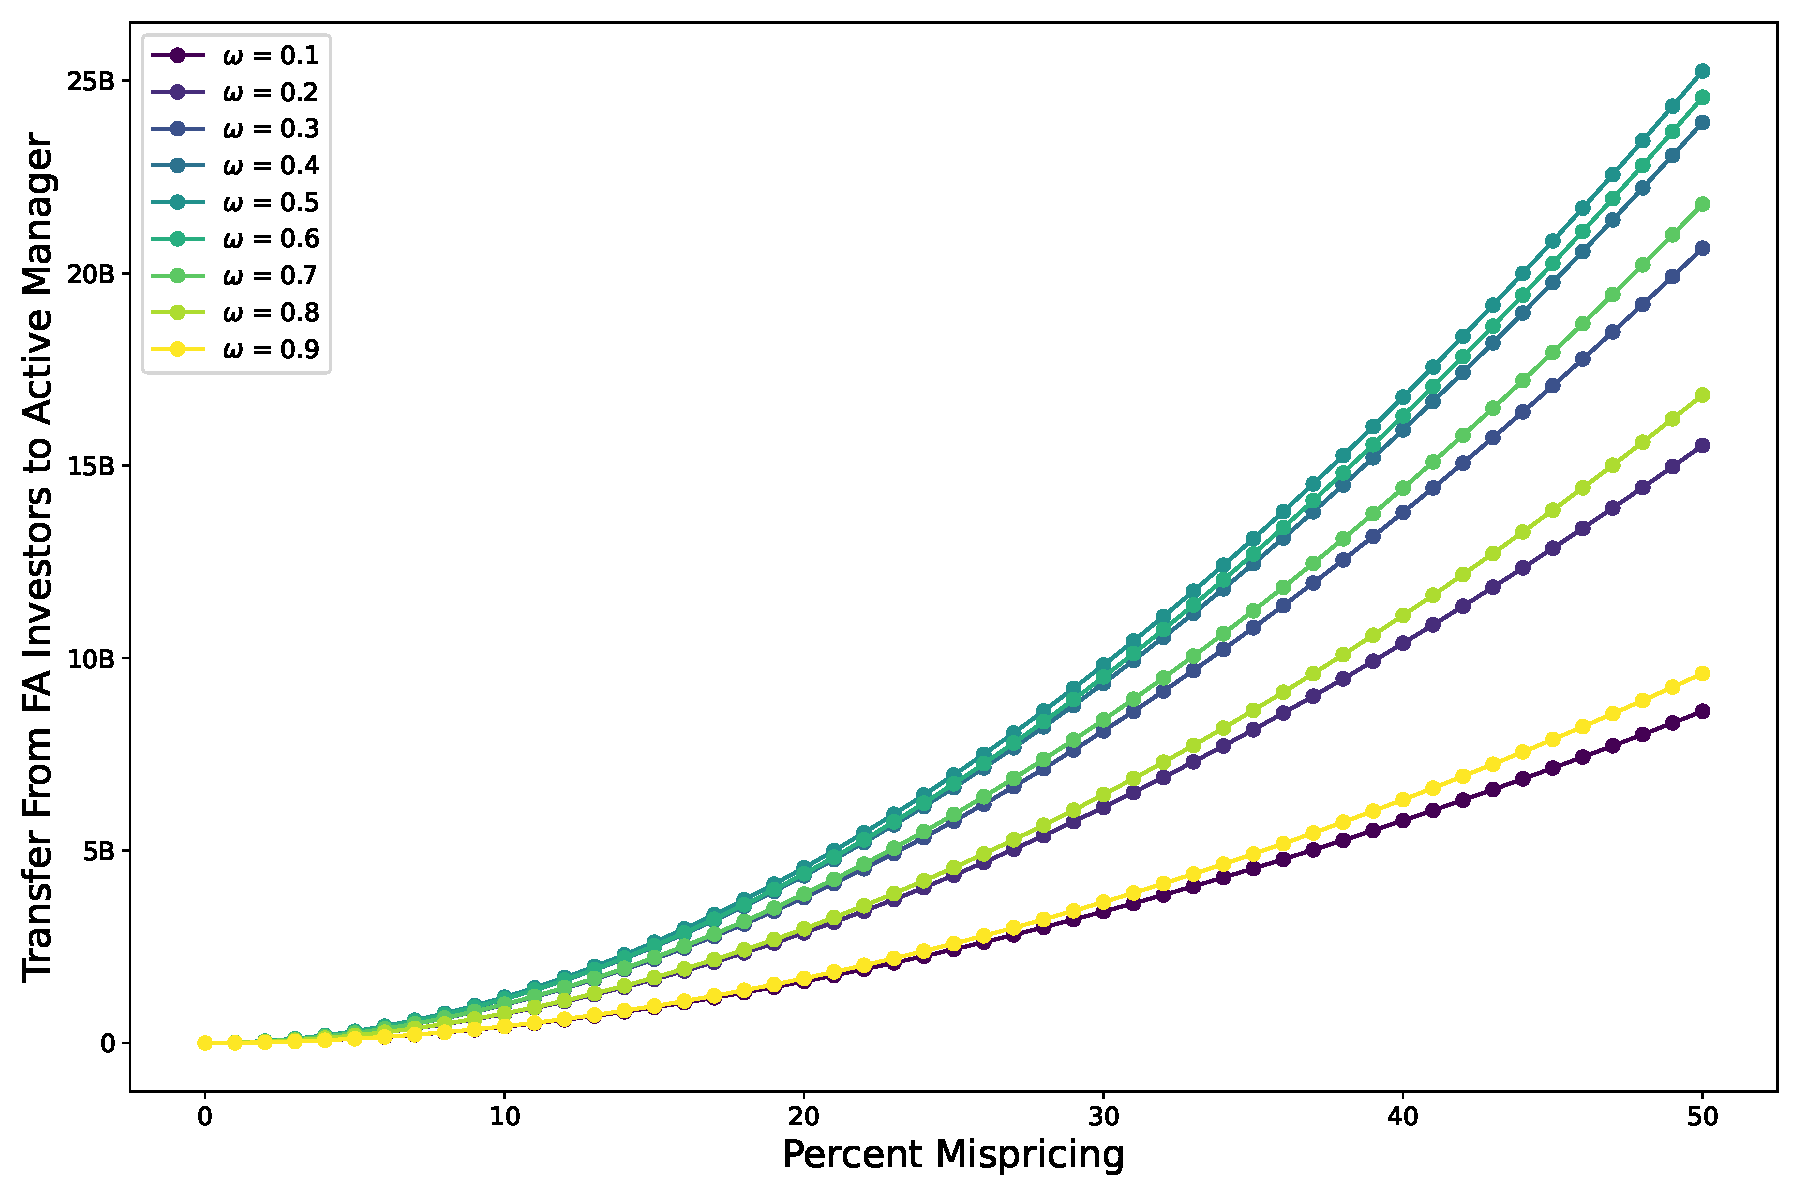
\includegraphics[width=\textwidth]{figures/profit_vs_mispricing_different_omegas.pdf}
    \begin{spacing}{1}
{\parbox{.95\linewidth}{
		\scriptsize{\scriptsize{{\emph{Notes}: Author's calculations. This figures illustrates the theoretical transfer from FA investors to active managers. I assume that the fixed allocation investors start with 1T in assets and $K=.0001$. $\omega$ refers to the share of the portfolio they seek to hold in the risky asset. Percent mispricing refers to the percentage change between the private price and the market price.  }}}}}
\end{spacing}
    \label{fig:profit_mispricing}
\end{figure} To conclude, small mispricings could compound to yield significant transfers, or rarer big mispricings could on their own create large transfers.

\section{Empirics} \label{sec:empirics}
The model presented above predicts that market responsiveness to informed trading should decrease as AUM in fixed allocation strategies increase. In other words, the fixed allocation investor acts as a na\"{\i}ve market maker providing greater liquidity. This decrease in market responsiveness should lead to higher profits for active managers, if private information quality stays the same. In this section, I measure the profits of active managers using the methodology of \citet{BERK2015}. I then present a measure of private information quality over time. 

Section \ref{subsec:active_proftis} measures and analyzes mutual fund value added. Section \ref{subsec:decomposition} examines the quality of private information over time.


\subsection{Does Rebalancing Enhance Active Manager Profits: Analysis of Mutual Fund Returns} \label{subsec:active_proftis}

To measure active manager returns, I turn to mutual fund return data from the CRSP Survivorship Bias U.S. Mutual Fund database \citep{Carhart}. Mutual fund value added was measured by multiplying alpha before fees by AUM \citep{BERK2015}. I determine the benchmark portfolio by regressing a mutual fund's monthly returns on the returns of Vanguard indices with year fixed effects to allow mutual fund alpha to evolve over time. Excess returns are computed by subtracting off the return of the benchmark portfolio. In Figure \ref{fig:active_passive}, we see that active manager value added has stayed relatively constant, as active manager AUM has risen. In Figure \ref{fig:passive_share}, I plot the value added of active mutual funds against the passive share of the market. This illustrates that despite the rise in passive investing share, the mutual fund value added has stayed relatively constant. Thus, the mutual value added has not grown while the fixed allocation investing strategy share has grown. Because fixed allocation investing did not take off until after the passage of the Pension Protection Act in 2006 \citep{vanguard20years}. Figure \ref{fig:passive_share} shows the trends before and after 2006. Holding private information quality and market responsiveness fixed, my model would predict that active mutual fund value added would increase due to taking advantage of the rebalance flows. 

\begin{figure}[htbp]{}
    \centering
    \caption{Total AUM in Active vs. Passive funds (1975 to 2023)}
    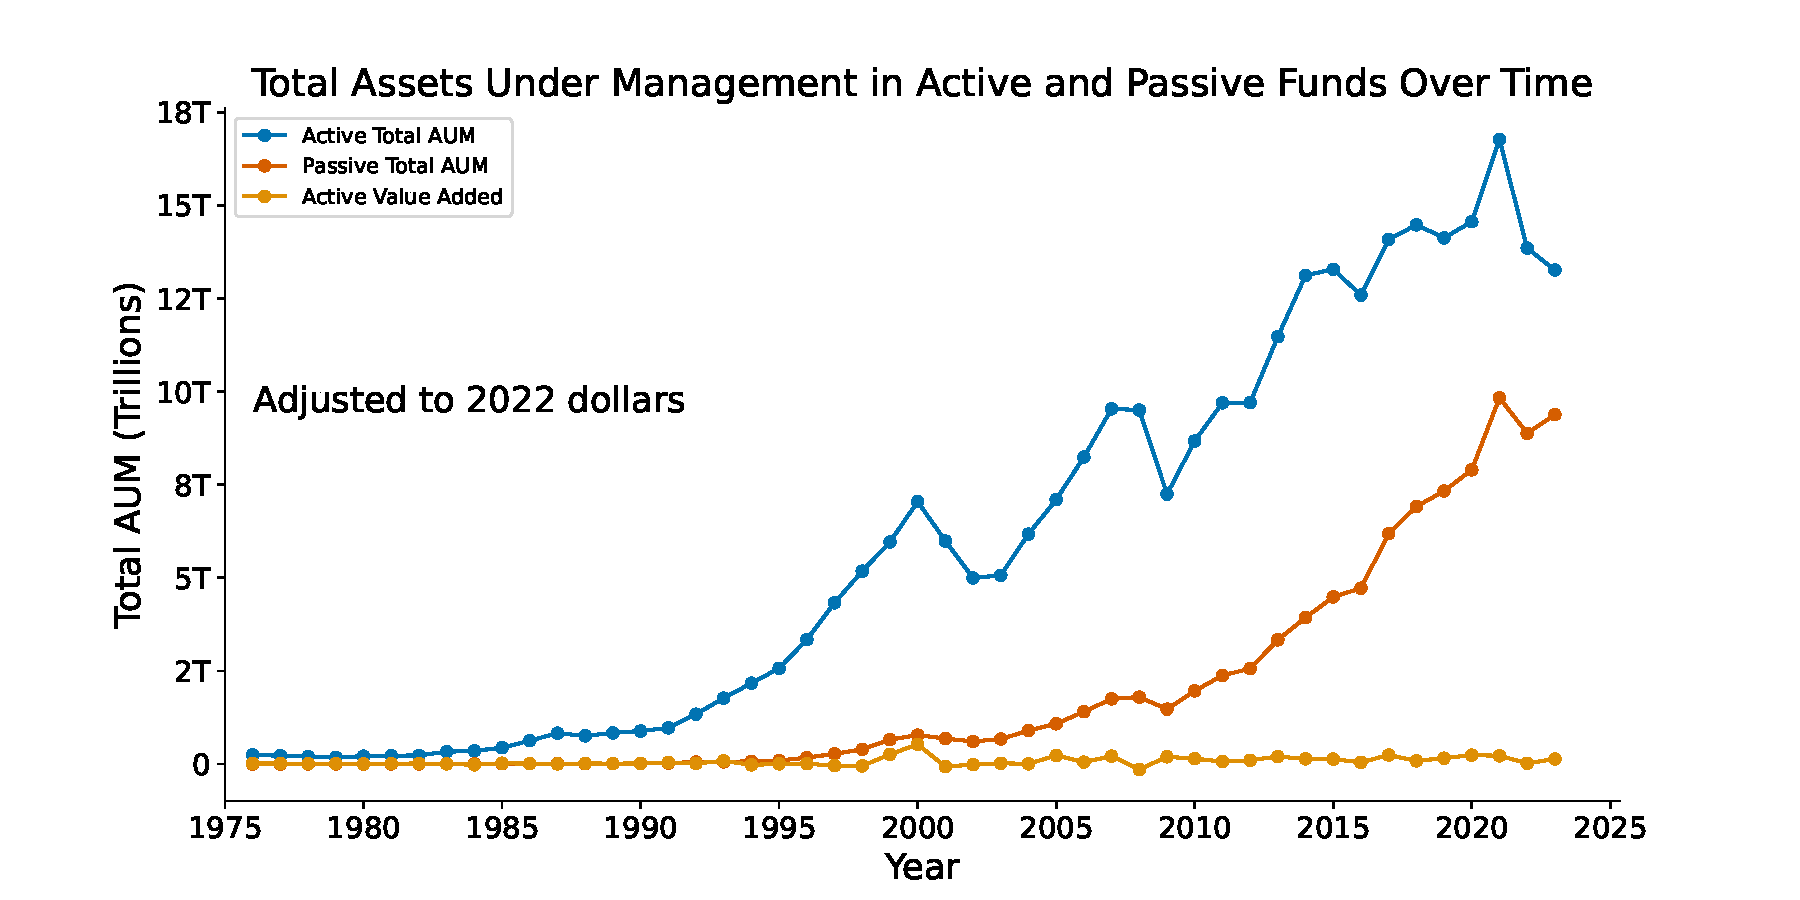
\includegraphics[width=\textwidth]{figures/active_passive_aum.pdf}
    \begin{spacing}{1}
{\parbox{.95\linewidth}{
	\scriptsize{\scriptsize{{\emph{Notes}: Author's calculations based on CRSP Mutual Fund Database. This figure depicts the assets under management in both active and passive mutual funds. I also show the value added from active mutual funds over my constructed vanguard benchmark. All values shown are in 2022 dollars. }}}}}
\end{spacing}
    \label{fig:active_passive}
\end{figure}
% Second Figure
\begin{figure}[H]{}
    \centering
    \caption{Active Funds Value Added vs. Passive Share of AUM}
    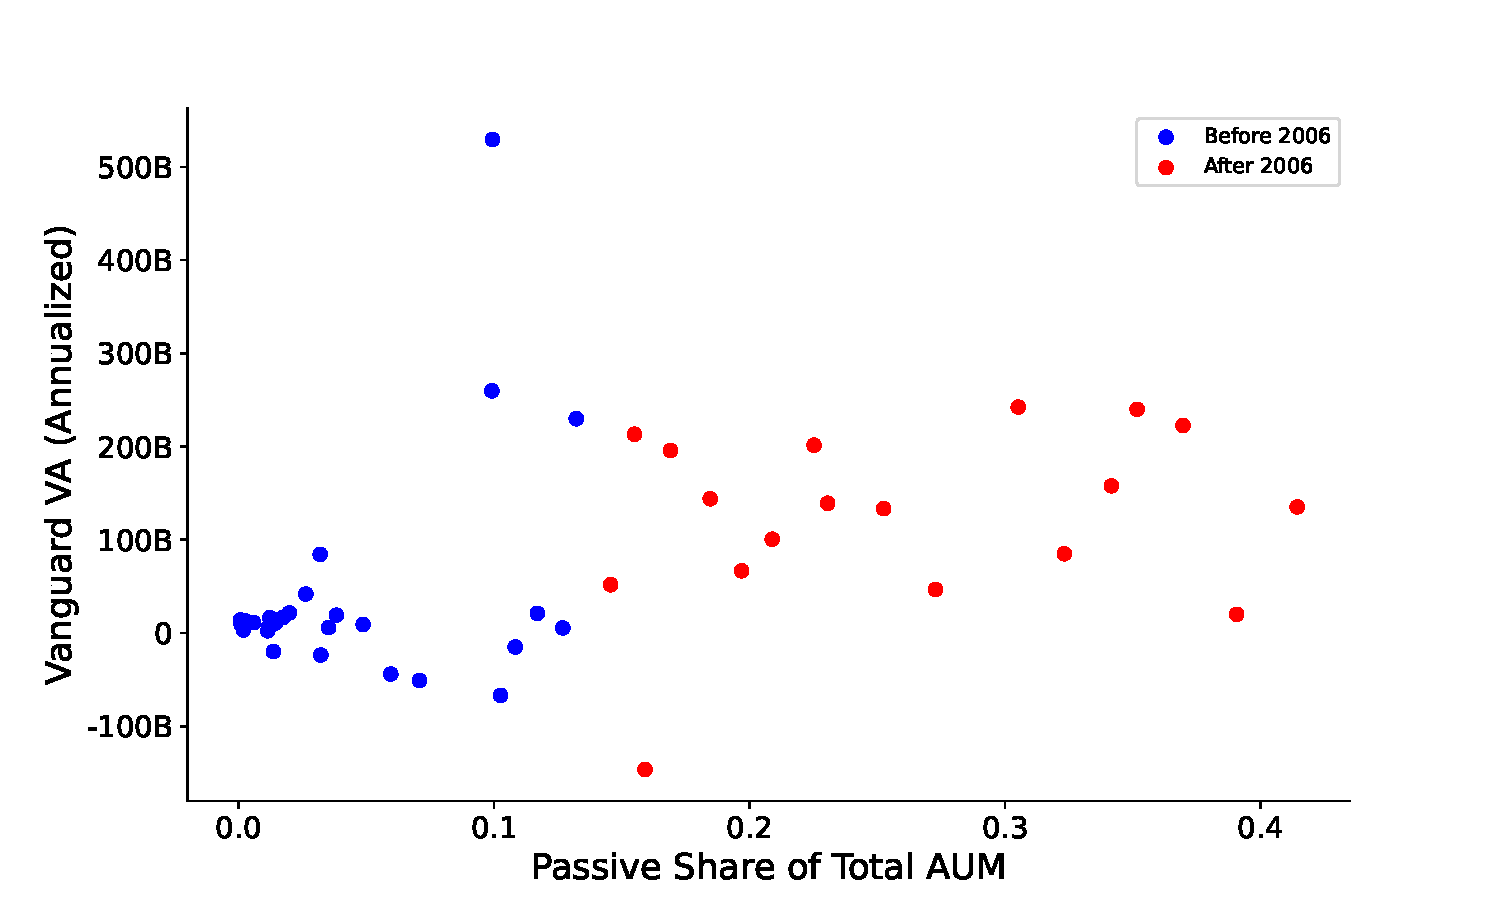
\includegraphics[width=\textwidth]{figures/active_passive_share_vanguard_va_pre_post.pdf}
    \begin{spacing}{1}
{\parbox{.95\linewidth}{
	\scriptsize{\scriptsize{{\emph{Notes}: Author's calculations based on CRSP Mutual Fund Database. This figure illustrates the value added of active mutual funds, using a constructed benchmark portfolio of Vanguard indices, against the share of the market in passive funds. Points in blue are from years before 2006 when the Pension Protection Act was passed. Points in red denote post 2006, when target date funds started to meaningfully gain market share. }}}}}
    \end{spacing}
    \label{fig:passive_share}
\end{figure}


\subsection{Decomposition of Mutual Fund Value Added} \label{subsec:decomposition}
To explore the basis for this surprising flatline in mutual fund value added,
I reason that the profitability of a mutual fund can be decomposed into 1) the quality of their private signals and 2) how quickly the market responds to their trade.
\begin{equation}
    \text{Value Added} = \sum_i (P_{private} - P_{i}) \ \forall \ i \quad s.t. \ P_{private} > P_i
\end{equation}
Assume that prices increase by a constant $K$ for each share purchased, i.e., $P_i = P_0 + iK$. Observe that $P_{private} - P_i$ will be positive for the first $n=\left\lceil \frac{P_{private} - P_0}{K}\right\rceil$ terms. If we can trade fractional shares we can omit the ceiling function.
\begin{align*}
    \text{Value Added} &= \sum_{i=0}^{n} (P_{private} - P_{i})\mathbbm{1}\{P_{private} > P_i\} \\
    &= \sum_{i=0}^{n} (P_{private} - (P_0 + iK)) \\
    &= n(P_{private} - P_0) - K\sum_{i=0}^n i \\
    &= n(P_{private} - P_0) - K\frac{n(n+1)}{2}
\end{align*}

\citet{CFM} show that mutual fund manager investments in firms where they have social connections perform better. This suggests that a major source of mutual fund value added is due to connections with company executives \citep{CFM}. To gauge the quality of this source of information, I track the profitability of company insider transactions through SEC form 4 filings from the Thomson Reuters Insiders Database. It is important to note the rules and regulations surrounding form 4 filings. Legally, company insiders must not trade on non-public information. For instance, the CEO of a company cannot buy shares moments after signing a huge deal for the company before the company announces the information. In other words, company insiders can only trade on public information. Like any individual, a company insider only trades for two reasons: hedging or a perceived mispricing. Company insiders typically hold large positions in their portfolios through equity compensation. I focus on insider purchases as sales are much more likely to reflect hedging rather than mispricing. If a company executive adds to their already large position in their own firm, they must expect a return large enough that it is worth forgoing the diversification benefits of purchasing a basket of stocks. I proxy this basket of stocks by using an ETF in the stock's sector assigned by the Thomson Reuters database. For each insider transaction, I use CRSP to compute the 6 month cumulative return (including dividends) from the day of the insider purchase. The excess return is defined as the return on the insider trade after 6 months net of the return of the benchmark ETF over the same time period. Accordingly this excess return acts as a proxy for the quality of private information in a given year. Figure \ref{fig:mean_net_ret_by_year} shows how this excess return measure has decreased significantly over time.
\begin{figure}[H]
    \centering
    \caption{Insider Transaction 6mo Excess Return By Year}
    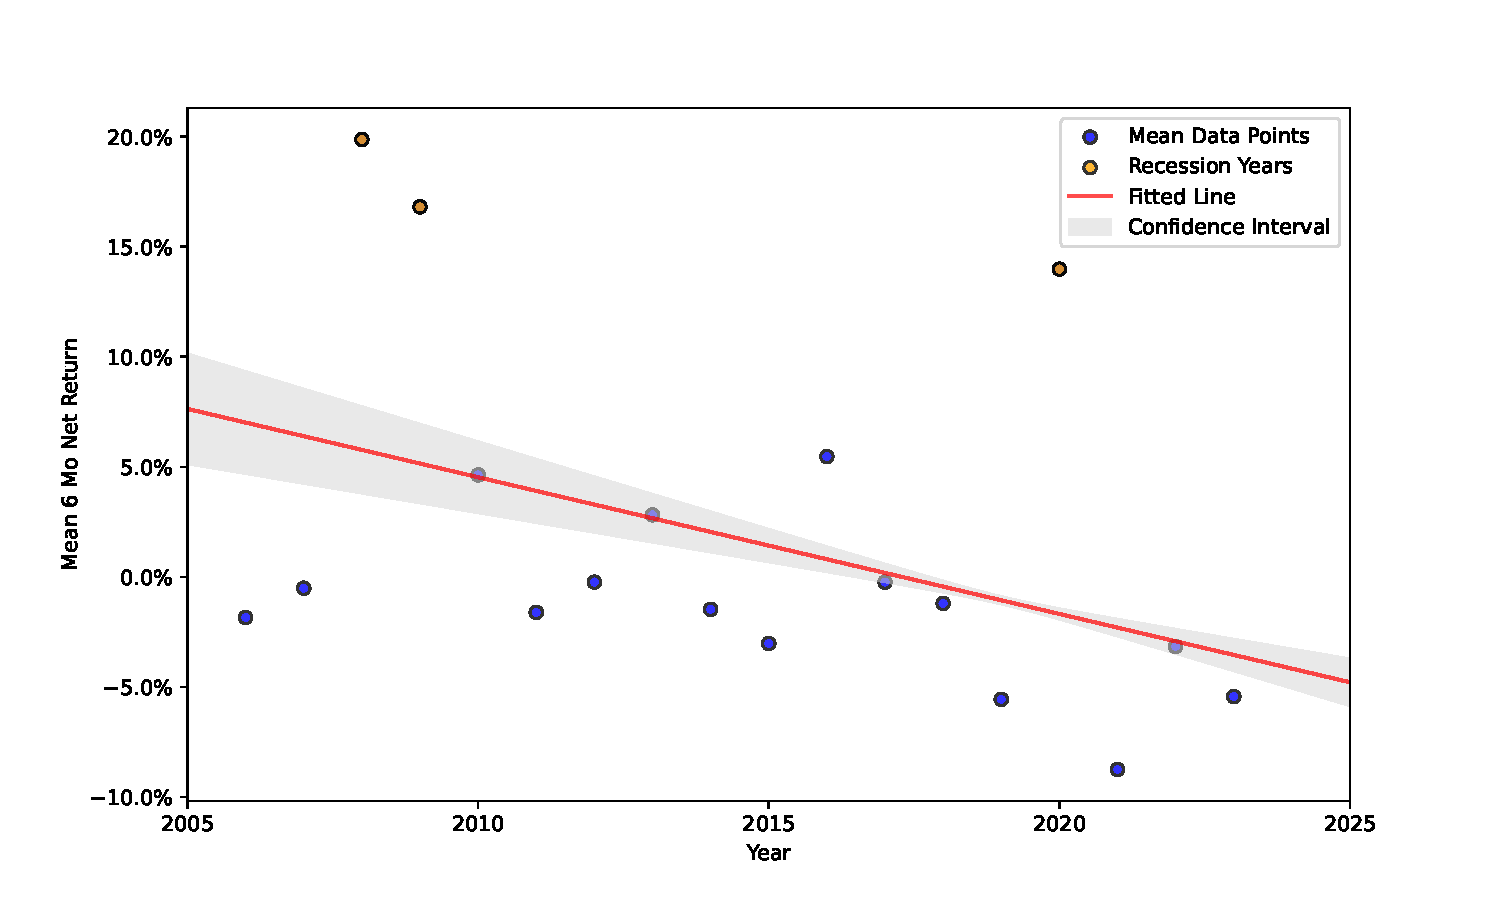
\includegraphics[width=\textwidth]{insider_trades/figures/mean_excess_ret_by_year_errors_recession.pdf}
\begin{spacing}{1}
{\parbox{.95\linewidth}{
		\scriptsize{\scriptsize{{\emph{Notes}: Author's calculations based on database of SEC form 4 filings. This figure illustrates the mean 6-month net return of insider transactions by year from 2006 to 2023. Each point represents the average 6 month excess return for a given year. The grey dashed line depicts the fitted regression line computed on the underlying data. The light grey band surrounding the fitted line denotes a 95\% confidence interval with clustered standard errors to account for the mechanical correlation from insiders making multiple trades in the same month. The points representing years 2008, 2009, and 2020 recessionary periods marked by high volatility are marked in yellow. Refitting the line excluding the recessionary years still yields a negative slope as shown in Appendix Table \ref{tab:regression_results}.}}}}}
\end{spacing}
    \label{fig:mean_net_ret_by_year}
\end{figure}
In Appendix Table \ref{tab:regression_results}, I show the results of a regression of excess returns on year at the trade level with clustered standard errors. I find that returns to insider transactions are fairly low and have declined over time. There are notable exceptions to this pattern during times of turmoil in markets. I further explore this pattern in Appendix Figure \ref{fig:vol}, showing the relationship between the CBOE S \& P 500 Volatility index and insider returns. Overall, declining returns to insiders trades suggest more difficult market environment for active managers. This aligns with my previous results about mutual fund value add, namely it has stayed relatively constant. As per my theoretical model, without private information, an active manager cannot profit.


\section{Conclusion} \label{sec:conclusion}
\par In this paper, I explore the implications of the rising prominence of fixed allocation investment strategies, particularly as they relate to asset pricing and the dynamics between passive and active management. My theoretical model suggests that while fixed allocation strategies may appear rational from a mean-variance optimization perspective, they inadvertently create opportunities for active managers to exploit, through rebalancing flows that mechanically ignore fundamental values.

\par My empirical analysis, however, reveals a surprising trend: despite the increasing assets under management (AUM) in passive strategies, the profitability of active mutual fund managers has not increased significantly. Instead, I find relatively flat mutual fund value added over time, suggesting that the anticipated opportunities for profit predicted by theory have not materialized.

\par To better understand this discrepancy, I decompose mutual fund value-added into private information quality and market responsiveness. The evidence from insider transaction data indicates that the quality of private information, as gauged by the profitability of insider trades, has diminished over the years. This decline suggests that more information is incorporated into prices today than in the past. Thus, if prices incorporate all available information there is no opportunity to transfer returns from fixed allocation investors to active investors.

\par In conclusion, I find that even though the growth of fixed allocation investing carries the potential to create a transfer to active managers, this has not materialized. However given the rapid rise of fixed allocation strategies, it is important to stay vigilant monitoring their performance in safeguarding the returns of the millions of Americans who are automatically enrolled in target date funds.
\newpage 

\bibliography{mybibliography.bib}
\newpage
\appendix
\section{Appendix}


\begin{table}[H]
    \centering
    \caption{OLS Regression Results}
    \label{tab:regression_results}
    \begin{tabular}{lrrrrrr}
\toprule
 & coef & std err & z & P>|z| & [0.025 & 0.975] \\
\midrule
const & 12.530700 & 1.821000 & 6.882000 & 0.000000 & 8.962000 & 16.099000 \\
x1 & -0.006200 & 0.001000 & -6.888000 & 0.000000 & -0.008000 & -0.004000 \\
\bottomrule
\end{tabular}

\end{table}

\begin{figure}[H]
    \centering
    \caption{Volatility and Insider Excess Returns Over Time}
    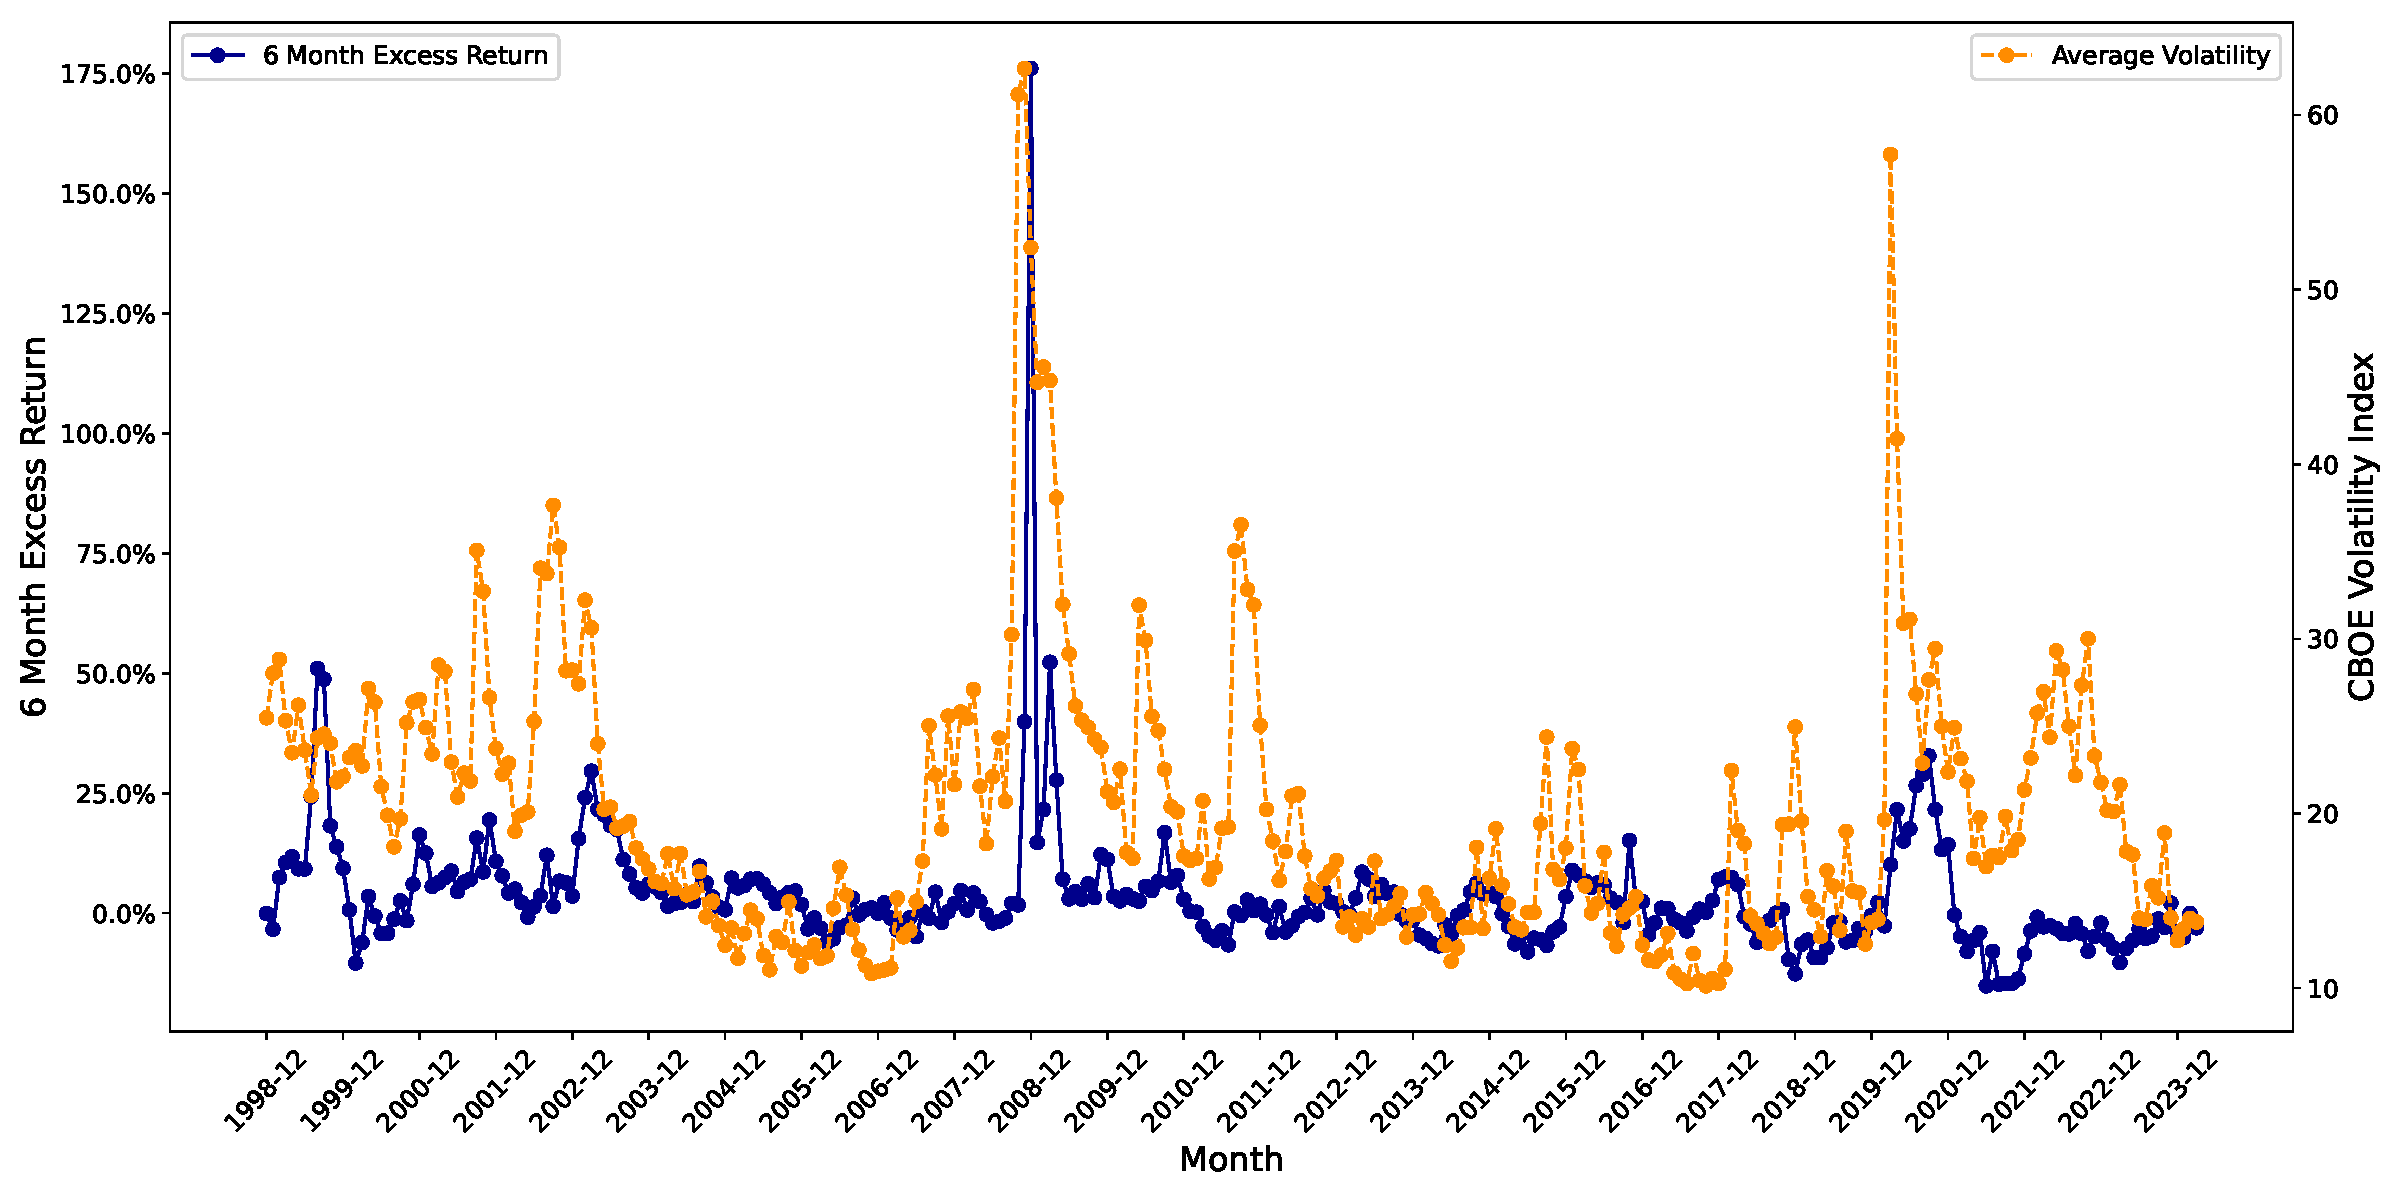
\includegraphics[width=\textwidth]{insider_trades/figures/vol_returns.pdf}
\begin{spacing}{1}
{\parbox{.95\linewidth}{
		\scriptsize{\scriptsize{{\emph{Notes}: Author's calculations based on database of SEC form 4 filings. This figure illustrates the mean 6-month net return of insider transactions by month from 1998 to 2023 plotted in blue. Each point represents the average 6 month excess return for a given month. The orange series depicts the average S \& P 500 Volatility index from CBOE.}}}}}
\end{spacing}
    \label{fig:vol}
\end{figure}

In graduate school, I am interested in exploring this relationship further. While low returns to insider information suggest market efficiency, there are notable exceptions during periods of turmoil, as measured by the VIX. This relationship is confounded by the macroeconomy, which the VIX reflects. I'm interested in determining whether uncertainty alone facilitates opportunities for sophisticated investors to profit. I want to examine how volatility at the individual stock level, measured through options pricing, conditional on the VIX, relate to returns from insider trading to better understand this dynamic. Hopefully, this will provide clues about market mispricing and how information makes its way into prices.


\section{Theory Appendix} \label{sec:theory_appendix}

Plugging in equations \eqref{eq:simple_unchar_demand} and \eqref{eq:simple_naive_demand} into equation \eqref{eq:supply_demand}, defining $W=W_{U,0}+W_{N,0}$, and combining terms yields the equation below.
\begin{equation}
    \frac{P_T-P_1^*}{(\gamma\sigma^2)^2}W\left(\frac{\mu_0}{P_0} + \frac{1-\mu_0}{P_1^*}\right) + \frac{P_T-P_1^*}{P_1^*\gamma\sigma^2}L - \frac{\mu_0}{\gamma\sigma^2}W\left(\frac{P_1^*}{P_0}\right) = 0
\end{equation}
I next multiply both sides by $\gamma\sigma^2$.
\begin{equation}
    \frac{P_T-P_1^*}{\gamma\sigma^2}W\left(\frac{\mu_0}{P_0} + \frac{1-\mu_0}{P_1^*}\right) + \frac{P_T-P_1^*}{P_1^*}L - \mu_0 W\left(\frac{P_1^*}{P_0}\right) = 0
\end{equation}
I next multiply both sides by $P_1^*$.
\begin{equation}
    \frac{P_T-P_1^*}{\gamma\sigma^2}W\left(\frac{\mu_0 P_1^*}{P_0} + 1-\mu_0\right) + (P_T-P_1^*)L - \mu_0 W\left(\frac{(P_1^*)^2}{P_0}\right) = 0
\end{equation}
I next rewrite in quadratic form.
\begin{equation}
(P_1^*)^2\left(\frac{-\mu_0W}{P_0}\left(\frac{1}{\gamma\sigma^2}+1\right)\right) + P_1^*\left(\frac{P_TW\mu_0}{\gamma\sigma^2P_0}-\frac{W}{\gamma\sigma^2}-L\right) + \frac{P_TW}{\gamma\sigma^2}\left(1-\mu_0\right) + P_TL= 0
\end{equation}
Plugging into the quadratic formula we get the expression below.
\begin{equation}
P_1^*= \frac{-\left(\frac{P_TW\mu_0}{\gamma\sigma^2P_0}-\frac{W}{\gamma\sigma^2}-L\right) \pm \sqrt{\left(\frac{P_TW\mu_0}{\gamma\sigma^2P_0}-\frac{W}{\gamma\sigma^2}-L\right)^2 - 4\left(\frac{-\mu_0W}{P_0}\left(\frac{1}{\gamma\sigma^2}+1\right)\right) \left(\frac{P_TW}{\gamma\sigma^2}\left(1-\mu_0\right) + P_TL\right)}}{2\left(\frac{-\mu_0W}{P_0}\left(\frac{1}{\gamma\sigma^2}+1\right)\right)}
\end{equation}


% \section*{Possible Extensions}

% \begin{itemize}
%     \item Solve for equilibrium between active and fixed allocation investors by assuming that the cost of a acquiring a signal is some function of its quality? Can I approximate the necessary parameters to predict what fraction of assets should be in fixed vs. active?
%     \item What would shift the equilibrium between active managers and fixed allocation investors?
%     \begin{itemize}
%         \item Cheaper Signals?
%         \item Changing risk aversion?
%         \item Changing Expected Risk Premia?
%     \end{itemize}
%     \item Does this imply that some fixed allocation investors should actually hold mutual funds?
% \end{itemize}

% \subsection*{Literature Review}

% \url{https://www.nber.org/system/files/working_papers/w12256/w12256.pdf}

% \url{https://pubs.aeaweb.org/doi/pdfplus/10.1257/jep.4.2.19}


% Idea here is to show that these constant allocation investors could encourage "boom-bust" cycles in a three period stylized model. At $t=0$ they are in equilibrium. At $t=1$, if the market goes up the levered investors become wealthier than the unlevered counterparts as their wealth appreciates faster than the unlevered investors. This means that subsequent moves in the market are amplified by their position (unlevered investors do not have the demand or supply to take the other side of the levered investors' trades). If the market moves down, the unlevered investors become comparatively wealthier as they lose wealth at a slower rate due to their lower risky asset exposure. This has a stabilizing effect as unlevered fixed allocation investors are "contrarians" meaning they buy when markets drop and sell when markets rise.

\newpage
% \section*{DEPRECATED - Fixed Allocation Investors Cannot Clear the Market Amongst Themselves}
% For simplicity, we consider a market with one risky asset (tangency portfolio or market index) and one risk-free asset (Treasuries, TIPS). Let there be a group of traditional investors (R) who are unlevered and a group of institutional investors (I) who hold a levered fixed percentage portfolio. Lastly, there are a group of arbitrageurs or fundamental investors who move the market exogenous to the fixed percent allocation investors. We examine this market through the lens of the fixed percent allocation investors maintaining their target allocation. These fixed-percent allocation investors demand or supply assets according to prices in the previous period (seek to "rebalance" according to the previous period prices). Since the prices are fixed from the previous period this induces an equilibrium between the traditional investors, R, and the institutional investors, I. Each investor has a weight $\omega_i$ on the risky asset and $1-\omega_i$ in cash. For an unlevered investor, $\omega_i \in (0, 1)$; for a levered investor, $\omega_i \in (1, \infty)$. In practice, one can only receive so much leverage, but imposing a maximum leverage does not change the model. Thus, the demand function for the risky asset of each investor is a function of their current cash position $C$, risky position $S$ and their desired risky weight $\omega$. 

% \[D(\omega, C, S) = \left(\omega - \frac{S}{S+C}\right)(S + C)\]
% I now consider the three possible cases for risky asset prices in two periods ($t=0$, $t=1)$.
% \subsection*{Risky Asset Stays Flat}

% At time $t=0$, the investor has their desired allocation i.e. $\frac{S_0}{S_0+C_0} = \omega$. If the risky asset stays flat, the investor does not need to trade as $S_0 = S_1$ and $C_0 = C_1$. This implies that $\frac{S_1}{S_1 + C_1} = \omega$, which is the desired allocation. 

% \subsection*{Risky Asset Moves}

% At time $t=1$, the market moves $K$ percent i.e. $S_1 = S_0(1+K)$. In this case, the investor needs to trade to "rebalance" their portfolio. Assume for simplicity, that the risk-free rate ($R_f$) is $0$. More generally, we can think of the return on the market as the excess return i.e. $K - R_f$. Thus, the person's wealth at $t=1$ is $W_1 = S_1 + C_1 = S_0(1+K) + C_0 = W_0(1+\omega K)$

% \begin{align*}
%     D(\omega, C_1, S_1) &= \left(\omega - \frac{S_1}{W_1}\right)(W_1) \\
%     &= \left(\omega - \frac{S_0(1+K)}{W_0(1+\omega K)}\right)(W_0(1+\omega K)) \\
%     &= \left(\omega - \omega\frac{(1+K)}{(1+\omega K)}\right)(W_0(1+\omega K)) \\
%     &= \omega\left(1 - \frac{(1+K)}{(1+\omega K)}\right)(W_0(1+\omega K)) \\
%     &= \omega\left(\frac{\omega K - K}{1+\omega K}\right)(W_0(1+\omega K)) \\
%     &= \omega K\left(\omega - 1\right)(W_0) 
% \end{align*}

% Before the market move ($t=0$), we assume that every investor has achieved their desired asset allocation i.e. $\frac{S_0}{S_0+C_0} = \omega$. If the market goes up, $K$ is positive i.e. $K > 0$. The retail investor $\omega \in (0, 1)$ in an up market must sell assets to maintain their desired asset allocation. At $t=1$, we show that the investor's demand is negative i.e. selling shares.
% \begin{align*}
%     D(\omega, C_1, S_1) = \omega K\left(\omega - 1\right)(W_0)
% \end{align*}
% When the risky asset goes up $K \%$, $W_0 > 0$ and $K > 0$. Thus, $D(\omega, C_1, S_1) > 0 \iff \omega > 1$. Therefore, levered investors demand assets, while unlevered investors supply assets. When the risky asset falls $K \%$, $W_0 > 0$ and $-1 <= K < 0$. $K$ is bounded below by $-1$ as equities are limited liability (they never go negative). Thus $D(\omega, C_1, S_1) > 0 \iff \omega < 1$. Therefore, unlevered investors demand assets, while levered investors supply assets. 


% \subsection*{Market Clearing Between Fixed Percentage Allocation Investors}

% Is there a way for levered and unlevered fixed allocation investors to clear the market exclusively trading with each other. In order for the market to clear, the supply and demand must be balanced. Our retail investors will be indexed from $1$ to $N$ with parameters $\omega_i, S_i, C_i$ and our levered investors will be indexed from $1$ to $M$ with parameters $\beta_j, S_j, C_j$. $\omega \in (0, 1)$ and $\beta \in (1, \infty)$. Since there is no supply or demand if the risky asset price stays constant, we consider the more interesting case where the risky asset moves $K \%$. We also assume that before the market move the investors have achieved their desired allocation $\omega$ (unlevered) or $\beta$ (levered). We then analyze the conditions that allow the market to clear.
% \begin{align*}
%     \sum_{i=1}^{N}D(\omega_i, C_i, S_i) + \sum_{j=1}^{M}D(\beta_j, C_j, S_j) = 0 \implies \sum_{i=1}^{N}D(\omega_i, C_i, S_i) &= -\sum_{j=1}^{M}D(\beta_j, C_j, S_j) \\
%     \sum_{i=1}^{N} \left(\omega_i - \frac{S_i}{S_i+C_i}\right)(S_i + C_i) &= -\sum_{j=1}^{M}\left(\beta_j - \frac{S_j}{S_j+C_j}\right)(S_j + C_j) \\
%     \sum_{i=1}^{N} \omega_i K (\omega_i - 1)W_{0i} &= -\sum_{j=1}^{M} \beta_j K (\beta_j - 1)W_{0j} \\
%     \sum_{i=1}^{N} \omega_i (\omega_i - 1)W_{0i} &= -\sum_{j=1}^{M} \beta_j (\beta_j - 1)W_{0j} 
% \end{align*}

% The key observation here is that in order for these fixed allocation investors to have no price impact (no unmet flows) they need to be in a precise balance. This likely isn't the case as after a market move levered and unlevered investors' wealth evolve differently. Thus, these fixed allocation investors cannot maintain this precise balance creating unmet flows that are independent of fundamental values (noise traders). Thus, other market participants must be trading with these fixed allocation investors.
\end{document}